\documentclass{article}
\usepackage[T1]{fontenc}
\usepackage{lmodern}
\usepackage{graphicx}
\usepackage{amsmath,amssymb}
\usepackage[a4paper,margin=2cm]{geometry}
\usepackage[absolute,overlay]{textpos}
\setlength{\TPHorizModule}{1mm}
\setlength{\TPVertModule}{1mm}
\usepackage[indonesian]{babel}
\usepackage{hyperref}
\setlength{\emergencystretch}{2em}
% unit: Halaman 32

\begin{document}

% === Halaman 32 (llm) ===

\textbf{1. Columnar Transposition Cipher}

\textbf{Contoh:} Misalkan plainteks adalah

\texttt{sistem dan teknologi informasi itb}

Panjang kunci = 6

\vspace{98.01mm}

\textbf{Enkripsi:}\quad\textcolor{red}{(*buang spasi)}

\vspace{40mm}

\textbf{Cipherteks: (baca secara vertical kolom per kolom)}

SDNIAIAONSSNLFITTOOIEEGRTMKIMB\quad\textcolor{red}{(tanpa spasi)}

SDNI AIAO NSSN LFIT TOOI EEGR TMKI MB\quad\textcolor{red}{(atau blok 4 huruf)}

% deskripsi: Ilustrasi proses enkripsi Columnar Transposition Cipher yang menunjukkan penyusunan teks ke dalam matriks dan arah pembacaan kolom menggunakan tanda panah biru.
% bbox normalisasi: [0.1100, 0.4700, 0.6700, 0.8000]
\begin{textblock*}{117.60mm}(23.10mm,139.59mm)
\noindent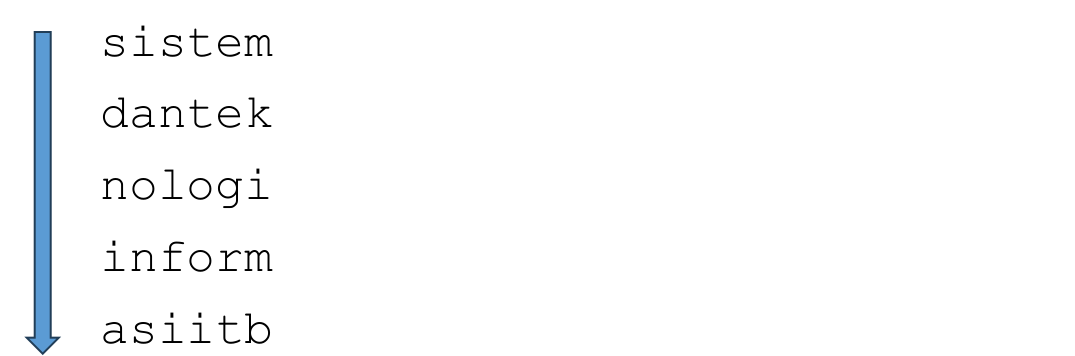
\includegraphics[width=117.60mm,height=98.01mm]{../../images/llm/page_032_img_01.png}%
\end{textblock*}

\end{document}
